\chapter{绪论}

\section{研究目的与意义}

当下,快节奏的生活方式催生出外卖配送、即时出行等需求,摩托车凭借其小巧灵活、通行便利的特性,在全球各地的城市交通体系中占据了愈发重要的地位。
无论是穿梭于大街小巷的外卖骑手,还是追求通勤效率的上班族,都将摩托车视为短途出行的首要选择。

市场需求的增长,有力推动了摩托车产业的蓬勃发展,其保有量在全国范围内持续攀升。但由于我国交通体系复杂、管理难度大以及驾驶人员安全意识淡薄,涉及摩托车的交通事故逐渐增多。头盔作为摩托车驾驶员和乘客最关键的防护装置,能有效缓冲撞击、减轻伤害,尽可能地保护驾乘人员的生命安全\cite{hss}。尽管国家出台了强制佩戴头盔的交通法规
来保障骑行者的生命安全,但部分骑行者安全意识淡薄,依旧心存侥幸,不佩戴头盔就上路行驶,如\ref{fig:traffic}。

当前,针对摩托车驾乘人员头盔佩戴情况的监管,主要依赖交警人工检查。然而,我国道路系统错综复杂,
交通流量庞大且情况瞬息万变,交警在维持交通秩序的同时,还要负责检查头盔佩戴情况,
工作负担极为沉重。人工检查不仅效率低下、耗费大量人力物力,而且在复杂路况和密集车流中,
极易出现漏检现象,难以确保监管工作的全面性和准确性。因此,一个摩托车驾乘人员头盔佩戴检测系统对减少人工工作量、提升检测速度和准确度有很大的意义。

\begin{figure}[!htb]
  \centering
  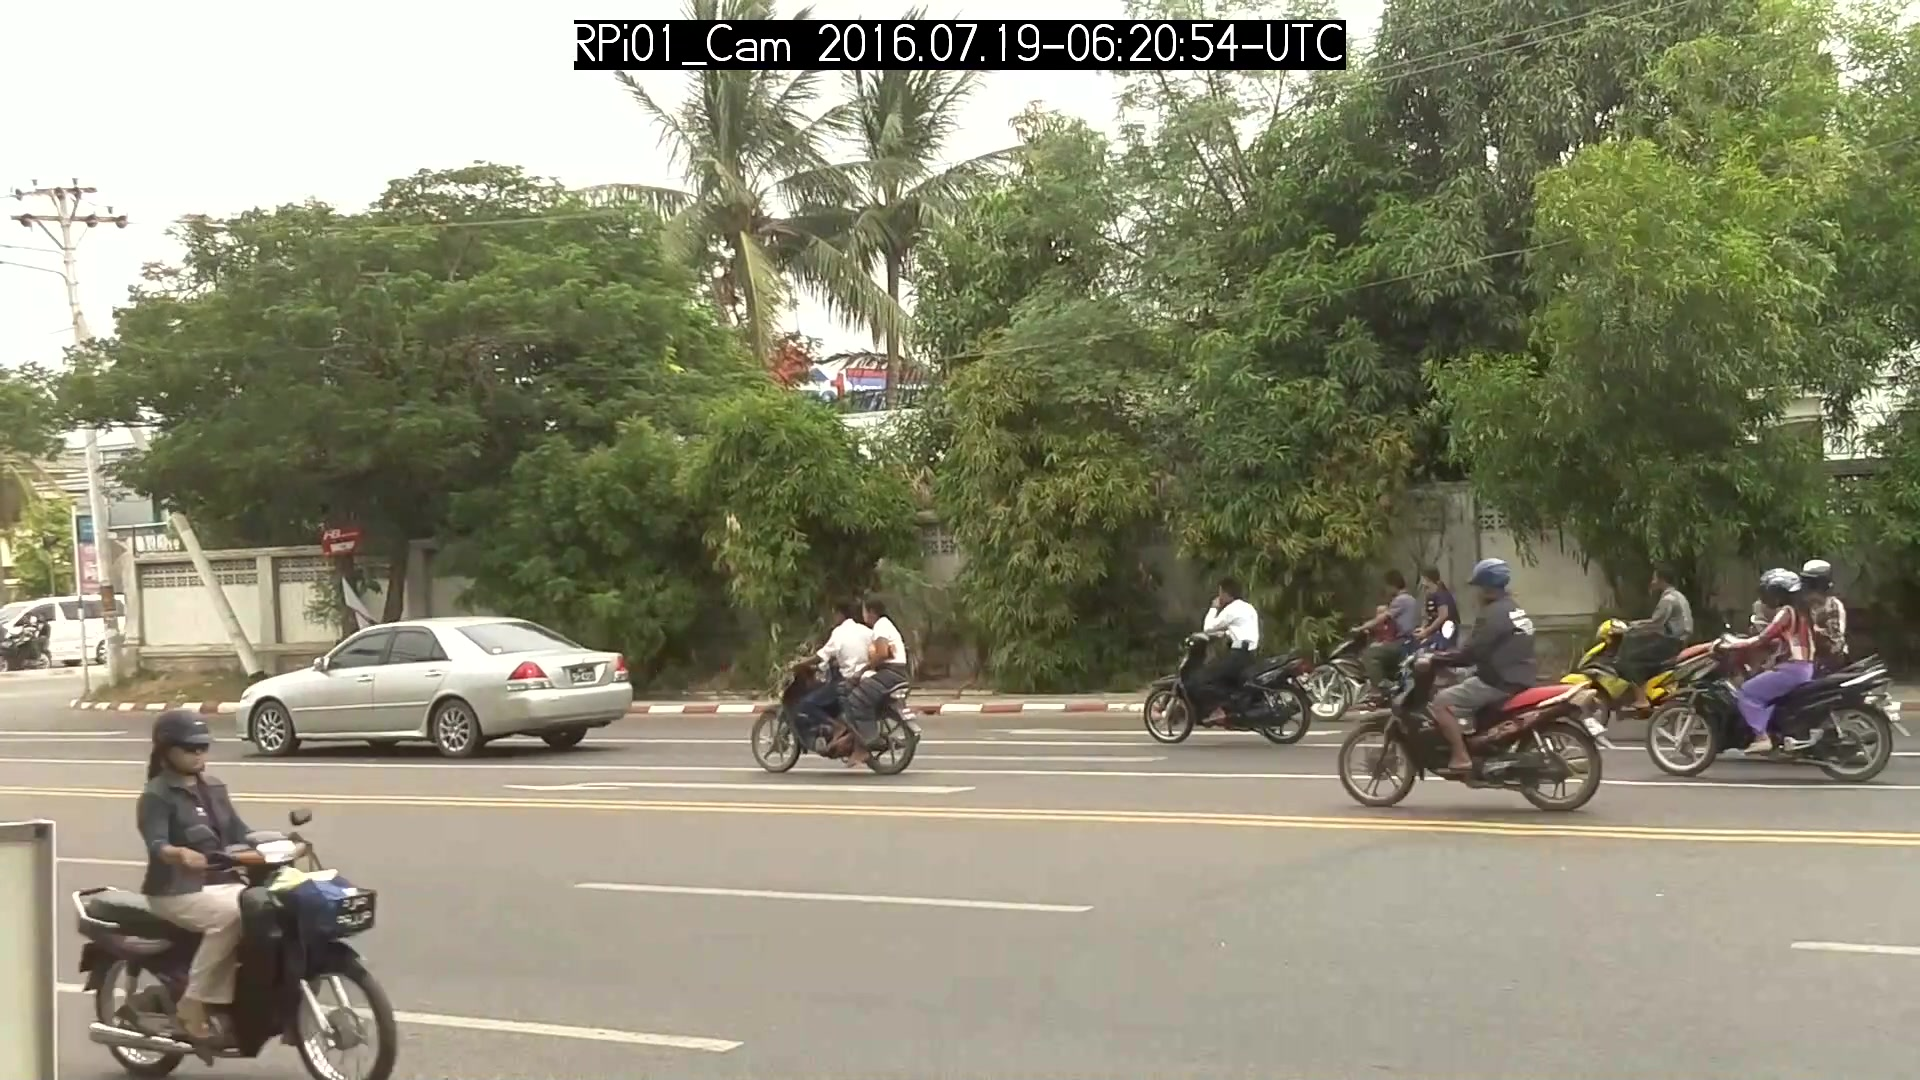
\includegraphics[width=0.85\textwidth]{figs/chap01/traffic}
  \caption{城市道路上摩托车驾乘人员头盔佩戴情况}
  \label{fig:traffic}
\end{figure}
\section{目标检测发展历程}

\ref{fig:his}(图像来源:\url{https://www.frontiersin.org/journals/built-environment/articles/10.3389/fbuil.2025.1563483/full})展示了目标检测的发展。

\begin{figure}[!htb]
  \centering
  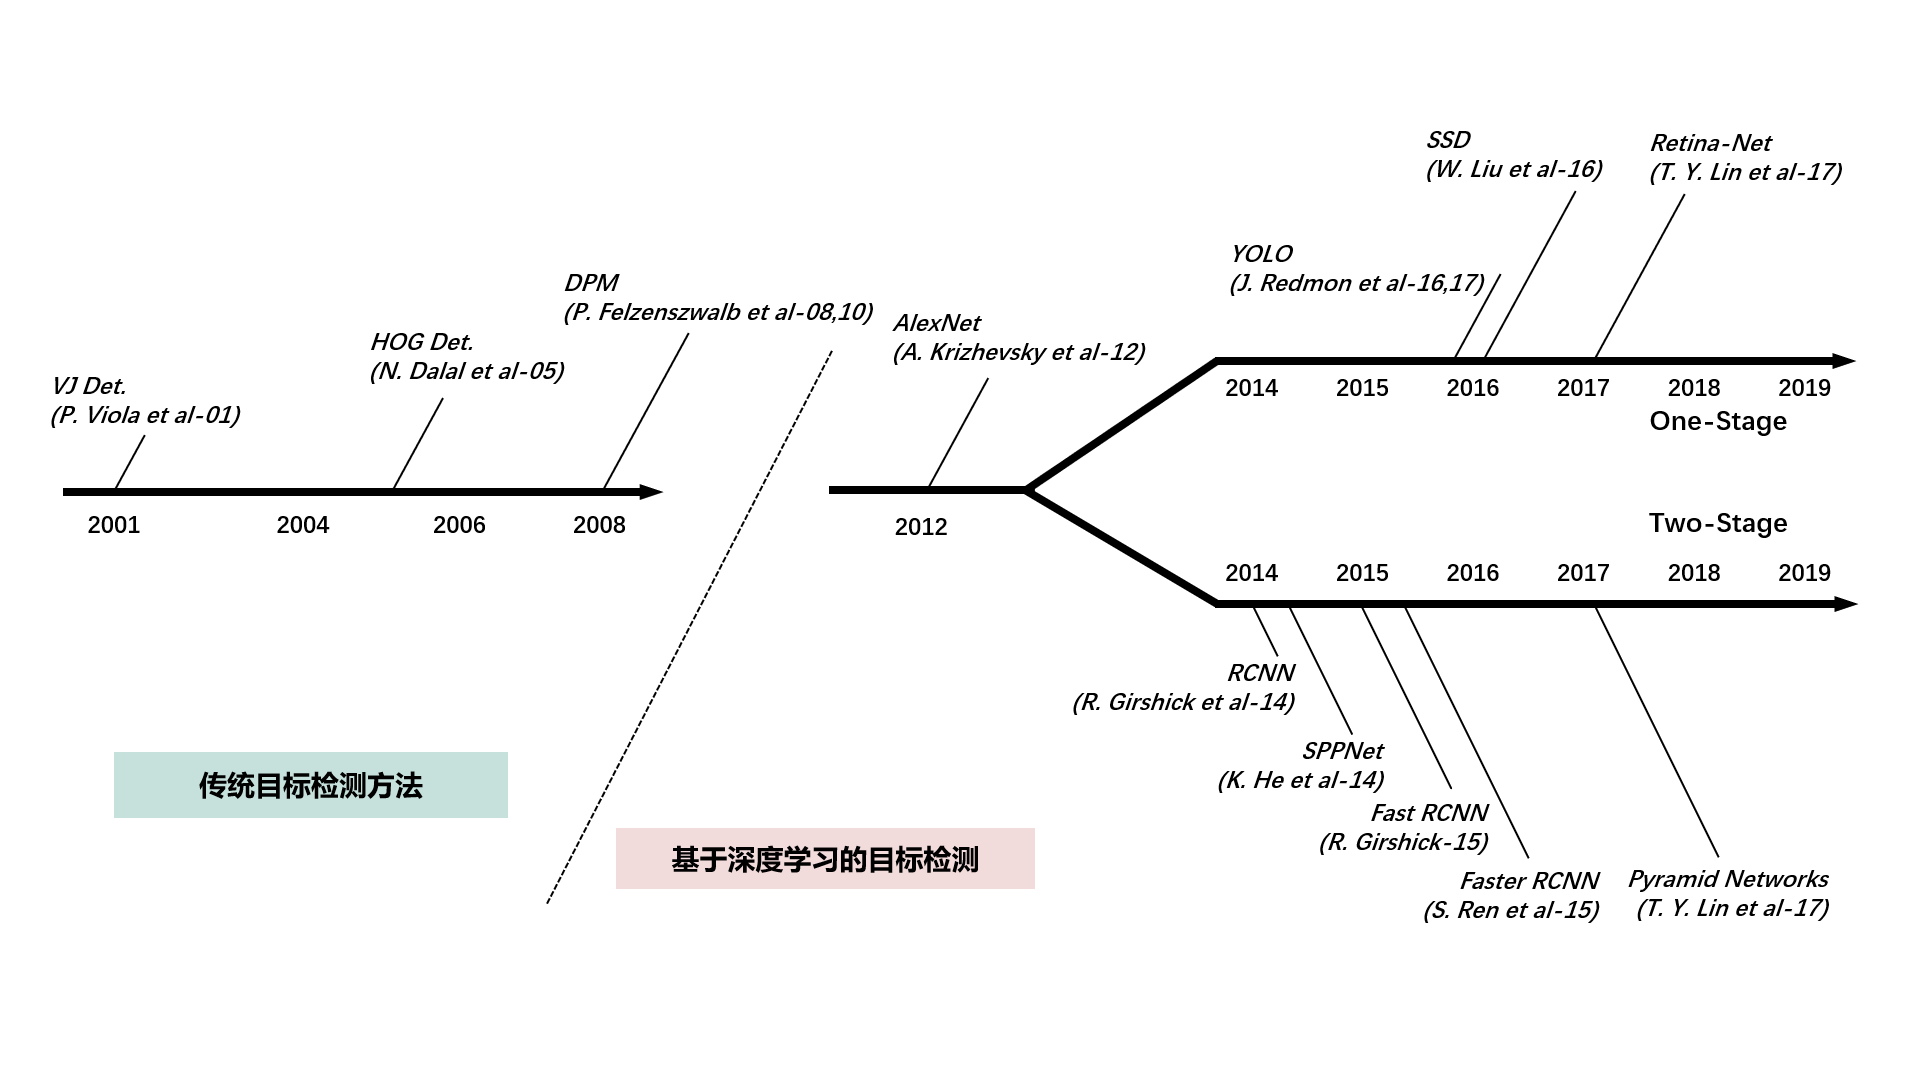
\includegraphics[width=0.9\textwidth]{figs/chap01/his.png}
  \caption{目标检测算法发展历程}
  \label{fig:his}
\end{figure}

\subsection{传统目标检测}
在深度学习兴起之前,受限于图像表示能力,研究者们需要设计复杂的特征表示。这一时期的代表成果深刻影响了后续目标检测技术的发展。

2001年,\textcite{Viola2001}首次在通用场景下实现了无约束的人脸实时检测。以两位作者命名的VJ检测器在检测精度没有损失的情况下,计算效率提高了1-2个数量级。该检测器运用滑动窗口,对图像内所有尺寸所有位置的窗口进行遍历,判别窗口中是否存在人脸。

Dalal与Triggs于2005年提出方向梯度直方图(HOG)描述器,对当时的尺度不变特征变换和形状语境做出重要改进\cite{Dalal2005}。HOG描述器最初针对行人检测任务而设计,以均匀分布的单元网格作为计算基础,引入重叠局部对比度归一化,显著提升了特征表征的准确性。该描述器应用于多尺度目标检测时,需保持检测窗口尺寸恒定,对输入图像实施多尺度变换以实现不同尺寸目标的识别。

DPM(Deformable Part Models)在目标检测领域具有重要地位,该模型最早由P. Felzenszwalb在2008年提出\cite{Felzenszwalb2008},是HOG检测器的优化版本,后续经R. Girshick等人不断优化改进\cite{Felzenszwalb2010Cascade}。

\subsection{基于深度学习的目标检测}
2012年,\textcite{alexNet}提出了一种经典的卷积神经网络AlexNet,它的出现极大地推动了深度学习领域的技术革新。目标检测算法依据其架构与运行机制,主要可划分为一阶段算法与两阶段算法两大类别。一阶段检测方法通过回归策略直接在输入图像上预测目标类别和空间位置,省去了候选框生成过程,提升了检测效率,使其适用于自动驾驶系统、智能视频监控等对实时性要求严苛的应用场景,典型代表包括YOLO系列和SSD等。两阶段检测方法首先生成潜在目标区域,随后对这些候选区域执行细粒度的分类和边界框回归,虽然这种分阶段处理机制能够获得更精确的检测结果,但不可避免地会使得目标检测的速度变慢。下面将对两阶段的代表算法R-CNN系列展开介绍,然后详细介绍本文使用到的一阶段的代表算法YOLO系列。

\subsubsection{R-CNN系列算法}
2014年,\textcite{rcnn}提出的R-CNN的思路为:
基于选择性搜索算法\cite{selectSearch}生成可能存在目标的潜在区域,并统一各区域的尺度。采用AlexNet网络架构对标准化后的候选区域进行深度特征提取,最后运用SVM对各个候选区域进行目标分类,实现对不同目标的准确识别与判定。该模型需对数量众多且相互重叠的候选区域(单张图像通常生成超过2000个候选框)进行特征提取计算,检测速度极慢。同年,\textcite{sppnet}通过引入空间金字塔池化层(SPP),突破了传统CNN需要固定输入尺寸的约束,能够输入任意尺寸图像并输出固定长度特征表示,将检测速度提升至R-CNN的20倍以上。

2015年,\textcite{fast-rcnn}提出了Fast R-CNN检测算法。该模型通过创新性地将检测器与边界框回归器集成于统一网络架构中进行联合训练,不仅显著缩短了模型训练和推理过程的耗时,同时使检测性能获得显著提升。

根据\textcite{faster-rcnn}的研究成果,Faster R-CNN检测器作为首个实现端到端训练的深度学习检测框架,在检测效率方面取得了突破性进展,首次达到了接近实时的检测速度。该模型通过创新性地引入RPN机制,显著提升了目标检测的运算效率与整体性能表现。RPN用于自动生成候选区域,在性能上要比选择性搜索算法好很多,推动目标检测系统从分散模块逐步整合为统一的端到端学习架构。

\subsubsection{YOLO系列算法}
2016年,\textcite{yolo}提出了YOLO算法,为目标检测任务提供了一种新的解决思路。其核心机制是利用单个卷积神经网络对整幅图像进行处理,将图像分割为多个区域后,直接预测各区域的边界框与对应类别概率,并通过概率加权对边界框进行筛选,经阈值处理后输出高置信度检测结果。YOLO算法显著提升了检测速度,但仍存在局限性:一是泛化能力弱,难以准确检测训练时未见过的新物体;二是空间约束大,每个网格单元仅预测两个框,不利于处理小目标群;三是定位误差大,经常误判物体位置。

YOLOv2是在YOLOv1发布一年后推出的\cite{yolov2},无论是分类还是检测,YOLOv2都比其前身YOLOv1有了很大的改进。YOLOv2的一大突破性进展在于开发了一种新的联合训练策略。该算法创造性地将检测数据集与分类数据集整合,使目标检测模型能够同时从两种类型的数据中获取信息,训练时同时提升检测精度与分类能力。通过标记检测图像学习目标精确定位,借助分类图像扩展模型识别类别范围、增强鲁棒性。



YOLOv3\cite{yolov3}基于YOLOv2进行改进与创新:一方面,YOLOv3修正了YOLOv2的数据加载缺陷,使模型平均精度均值(mAP)提升了两个点;另一方面,YOLOv3采用Darknet-53骨干网络,引入多尺度预测架构(三尺度特征金字塔)优化跨尺寸目标检测能力。

相较于YOLOv3,YOLOv4\cite{yolov4}在骨干网络和颈部网络两个关键环节进行了创新升级:骨干网络层面,摒弃原有架构,采用CSPDarknet53作为新的骨干网络,通过跨阶段部分网络(CSPNet)策略优化特征提取;颈部结构上,改进空间金字塔池化(SPP)与路径聚合网络(PAN)的引入,进一步强化多尺度特征融合能力。

YOLOv5较YOLOv4在易用性上实现了提升。除了性能上面一些微小的提升之外,YOLOv5基于PyTorch框架重构代码,简化了模型的部署,同时提供了更详尽的多语言文档支持,降低开发门槛。

YOLOv6是YOLO系列中的一次重大演变,由美团视觉团队开发\cite{yolov6}。YOLOv6对YOLOv4和YOLOv5里的PAN拓扑结构进行了强化,借助RepBlocks与CSPStackRep Blocks,更高效地从骨干网络的不同层级聚合特征。除此之外的创新还有:通过硬件感知架构设计与动态训练策略的协同创新,在速度精度平衡与部署效率层面实现突破性进展;核心架构采用EfficientRep主干网络,基于RepVGG重参数化思想构建分层模块化结构,显著提升GPU推理效率;特征融合模块重构为Rep-PAN拓扑,通过重参数化卷积增强跨尺度信息流,并结合解耦式预测头缩减冗余计算。

YOLOv7基于YOLOv6提出了一系列细粒度的改进\cite{yolov7}。提出计划的重新参数化模型,将梯度传播路径概念应用于不同网络层;针对多输出层模型训练,引入标签分配的新方法;创新性地构建了“扩展”与“复合缩放”两种新型策略,通过优化参数配置与计算资源分配机制,显著提升了目标检测模型的性能表现。这些改进和优化策略,在不牺牲速度的情况下显著提高了准确率,是YOLO系列的重要进步。

YOLOv8在检测精度和速度方面实现了更优的性能,延续了YOLOv5用户友好的特点,进一步增强了易用性。YOLOv8采用无锚分割Ultralytics head,提升了检测的准确性与速度。YOLOv8 由Ultralytics维护,提供了针对检测、分割、分类和姿势检测等特定任务的多种专用模型。

相较于前代模型,2024年提出的YOLOv9采用全新思路,解决了深度神经网络信息丢失的问题\cite{yolov9}。YOLOv9的核心创新在于两大关键技术:一方面,引入可编程梯度信息(PGI),通过辅助可逆分支完整保留输入信息,为目标函数计算提供充足依据,确保梯度更新更精准有效;另一方面,提出了ELAN架构的通用轻量化版本——GELAN,作为,基于梯度路径规划设计,最大化网络信息流,高效整合特征信息辅助预测。

同为2024年提出的YOLOv10相较于前代模型,刷新/了速度与准确度上限,实现了真正的实时检测\cite{yolov10}。YOLOv10的核心创新在于:一是采用NMS-Free检测,基于双重标签分配(一对多和一对一)及一致匹配度量的训练策略,推理时仅用一对一head,提升推理速度、简化部署、增强训练监督;二是运用整体效率-准确度驱动设计,通过轻量级分类head、空间通道解耦下采样和等级引导块设计,在优化模型各组件的同时有效降低计算成本。

2024年9月发布的YOLOv11历经一系列架构改良,聚焦于在无损检测准确性的前提下,全力提升计算效率。YOLO11创新性地引入了C3k2模块与C2PSA块等关键组件。C3k2模块作为跨阶段部分(CSP)瓶颈的高效计算实现,取代了骨干网络和颈部网络中的C2f块。C2PSA块紧跟SPPF模块之后,这种全新的注意力机制,使模型能够更为高效地聚焦于图像内的关键区域,精准识别目标物体。




% 2012 年,AlexNet的提出推动了深度学习在目标识别领域的广泛应用\cite{alexNet}。随后,R - CNN 系列\cite{rcnn}、
% Fast R - CNN\cite{fast-rcnn}、Faster R - CNN\cite{faster-rcnn} 等两阶段检测方法不断改进,显著提升了检测精度和效率。SSD 
% 和 YOLO 系列作为单阶段检测方法,以不同的方式实现了高效的目标检测。其中,YOLO 系列将
% 目标检测转化为回归问题,极大地提高了检测速度,并且后续版本不断优化,加入了多尺度训练等技术,
% 以应对不同尺寸物体的检测需求。

\subsection{YOLO在交通安全领域的应用}
YOLO系列算法凭借出色的检测速度和准确性在交通安全领域得到了广泛的应用。在车辆检测、行人检测以及道路检测方面均表现出强大的应用潜力。

在车辆检测方面,\textcite{ex1}基于YOLOv8算法,提出了结合Transformer结构全局特征提取能力的模块C2Former代替C2f模块,提升了算法在目标被遮挡场景下对交通车辆检测的精度。\textcite{ex2}针对雾天场景下的车辆检测需求,引入注意力模块(CBAM、NAM、SimAM)和BiFPN结构优化YOLO-V5s/V5l,并对比了YOLO-V5/V8系列模型的性能,优化了算法在雾天中对车辆的检测性能。

在行人检测方面,\textcite{ex3}基于YOLOv7将ELAN-SA模块与LGA模块相结合,增强了特征提取能力,在遮挡和小目标行人检测方面表现出很强的性能。\textcite{ex4}基于YOLOv11,融合RepConv来改进C3k2模块,设计全新的颈部结构MBFPN,提升特征提取与融合能力,提出了轻量化行人检测算法。

在道路检测方面,\textcite{ex5}提出基于YOLOv8n的轻量化改进算法 EMF-YOLO,通过引入增强型特征融合金字塔EFFPN、可变形注意力机制和多尺度边缘敏感性增强模块MESA等,实现了模型的轻量化。 

YOLO算法凭借其高效性与准确性,已在交通、工业、医疗等多个领域发挥其作用,提供了精准的实时监测能力,推动各个行业的智能化发展。

\section{研究与设计内容}
本文旨在设计并实现一套摩托车驾乘人员头盔佩戴检测系统,工作分为两个部分:模型训练和系统开发。

在模型训练阶段,主要开展两方面工作:
一是优化数据标注,针对驾驶员及最多三名乘客(训练数据集中,最多 只出现了一名驾驶员携带三名乘客)各自的头盔佩戴情况,细化设置了18个标签,相较于传统二分类标注,能提供更详尽的头盔佩戴信息;二是训练两个关键模型,分别用于识别摩托车驾乘人员的头盔佩戴状态,以及驾驶员id。训练过程中,采用YOLOv11n、YOLOv11s及YOLOv11m三种模型训练来比较效果,最后总结不同模型的优势与适用场景。

系统基于浏览器/服务器(B/S)架构开发。B端浏览器为用户提供了两个操作页面,一个是用于上传图像或视频以请求检测的页面,用户可通过该页面发起检测需求;另一个是数据查询页面,用户能从该页面向服务端数据库发送历史检测结果查询请求,还可以对驾驶人、记录时间、记录地点等字段进行过滤。查询得到的结果会以柱状图、折线图等可视化的形式在页面呈现,为后续制定执法策略提供数据支持。S端服务器负责处理浏览器传来的请求,当接收到用户上传的图像或视频后,先利用第一个模型预测图像中的头盔佩戴情况,之后对目标区域进行裁剪,再使用第二个模型检测目标区域的驾驶人员,并将检测结果保存到本地磁盘。\ref{fig:source}和\ref{fig:result}表示了输入图像和检测结果。

\begin{figure}[!htb]
  \centering
  \begin{minipage}{0.45\textwidth} % 调整宽度以适应需求,两张图总宽度接近1
      \centering
      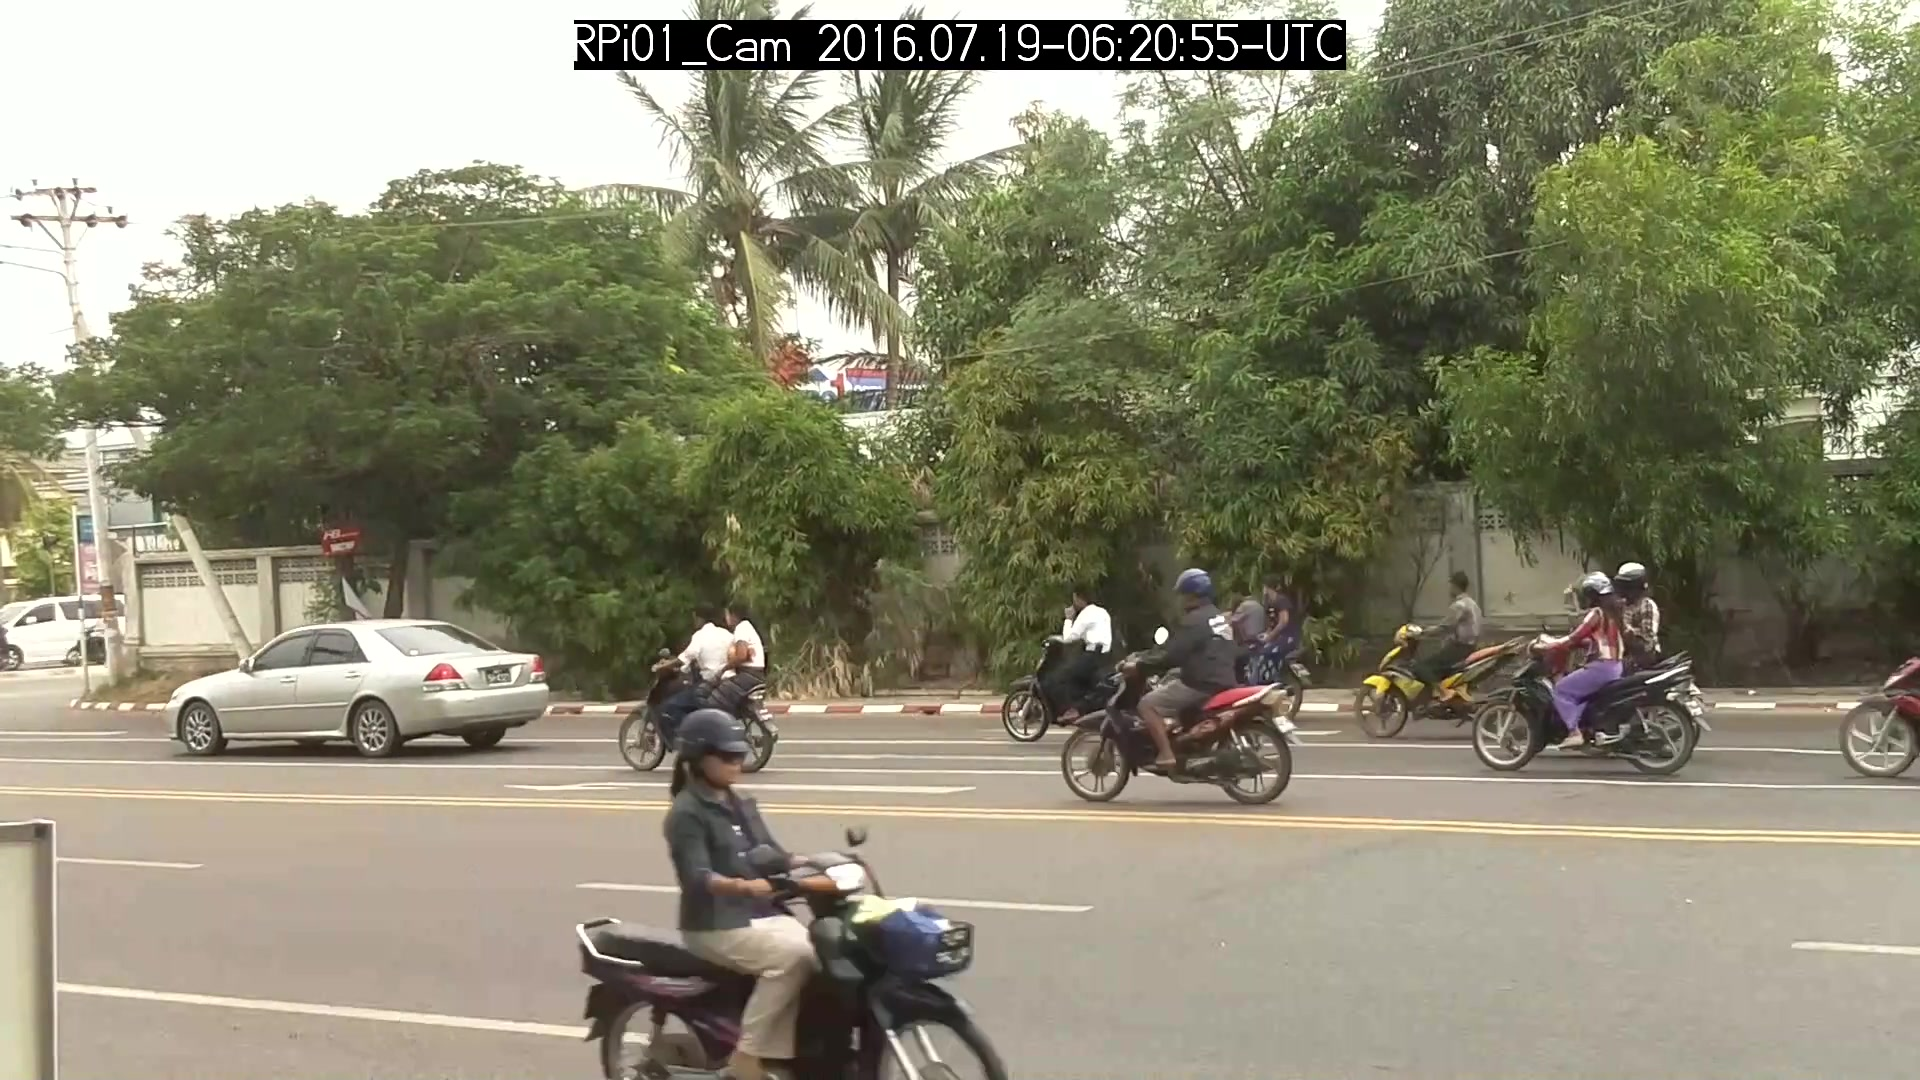
\includegraphics[width=\textwidth]{figs/chap01/source.jpg}
      \caption{输入图像}
      \label{fig:source}
  \end{minipage}
  \hfill % 使两张图像之间保持一定距离
  \begin{minipage}{0.45\textwidth}
      \centering
      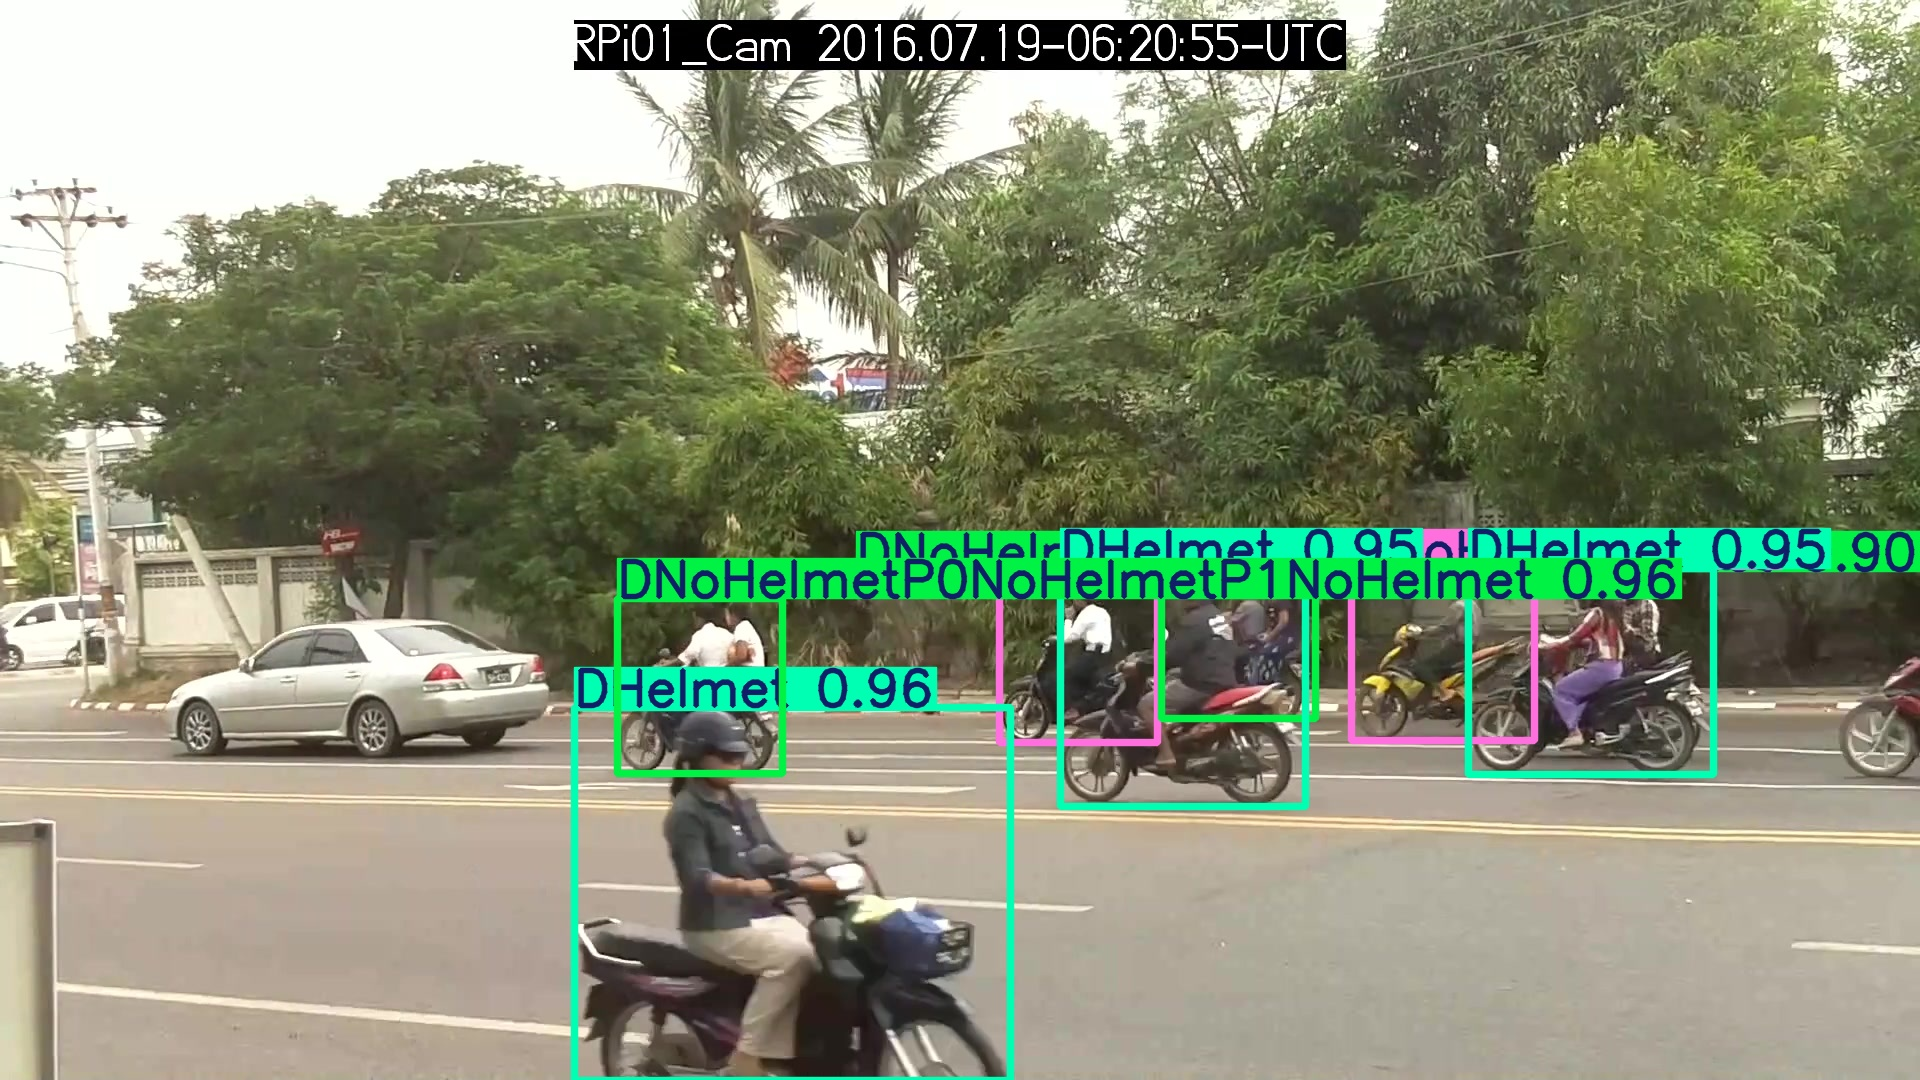
\includegraphics[width=\textwidth]{figs/chap01/result.png}
      \caption{检测结果}
      \label{fig:result}
  \end{minipage}
\end{figure}


\section{章节安排}
本文共包含六个章节,每一章的主要内容如下:

第一章:绪论。本章首先介绍了本文的研究目的与意义,对目标检测的发展历程进行概述,详细介绍了YOLO系列算法的发展过程及其在交通安全领域的应用现状,最后说明了本文的研究内容。

第二章:YOLO算法相关理论。本章深入阐述YOLOv11算法的核心构成,涵盖网络架构与损失函数两大关键模块。骨干网络通过C3K2和C2PSA两大创新点增强特征提取能力;颈部网络引入C3K2模块,并结合C2PSA模块的优点提升了特征融合能力;检测头以骨干网络和颈部网络生成的不同尺度的特征图像来生成预测框。损失函数主要介绍边界框回归损失函数、分类损失函数和分布损失函数。然后介绍了本文的数据集来源以及为解决类别不平衡对数据集做的增强处理,分析了增强之后的标签数量分布情况,然后介绍了实验所采用的硬件配置及软件环境,说明了模型训练过程中的具体参数设置。

% 第三章:数据集构建及训练参数设置。本章介绍了本文的数据集来源以及为解决类别不平衡对数据集做的增强处理,分析了增强之后的标签数量分布情况,然后介绍了实验所采用的硬件配置及软件环境,说明了模型训练过程中的具体参数设置。

第三章:实验结果与分析。本章首先介绍了本文使用到的目标检测模型检测精度和速度两方面的评价指标,展示了YOLOv11n、YOLOv11s和YOLOv11m这三个模型的训练结果,对比分析了上述三个模型的损失函数、精度、召回率、mAP以及检测速度。并总结了不同模型各自适用的场景。

第四章:检测系统的设计与实现。本章主要介绍了摩托车驾乘人员头盔佩戴检测系统的设计与开发过程。从需求分析、系统架构、前端模块开发和后端模块开发这四个方面展开。

第五章:总结与展望。本章为本文的最后一张,对本文所做的工作进行总结,并展望目标检测技术在交通安全领域的未来的发展情况。
%%% Local Variables:
%%% mode: latex
%%% TeX-master: "../main.tex"
%%% End:
